%=============================================================================
%  Z-Score Signal Generation — Mathematical Notes & Documentation
%  Study Notes + Technical Reference | Dark Wing Project
%=============================================================================
\documentclass[10pt,a4paper,twocolumn]{article}

%--- Geometry ----------------------------------------------------------------
\usepackage[a4paper,top=1.8cm,bottom=1.8cm,left=1.5cm,right=1.5cm,
            columnsep=0.7cm]{geometry}

%--- Math --------------------------------------------------------------------
\usepackage{amsmath,amssymb,amsthm,mathtools}

%--- Typography --------------------------------------------------------------
\usepackage[T1]{fontenc}
\usepackage{lmodern}
\usepackage{microtype}
\usepackage{parskip}
\setlength{\parskip}{2pt}

%--- Colours -----------------------------------------------------------------
\usepackage{xcolor}
\definecolor{codebg}{RGB}{245,247,250}
\definecolor{codeframe}{RGB}{180,195,220}
\definecolor{keyword}{RGB}{0,80,180}
\definecolor{comment}{RGB}{80,115,80}
\definecolor{string}{RGB}{160,40,20}
\definecolor{mathbluebg}{RGB}{230,240,255}
\definecolor{mathblue}{RGB}{10,60,160}
\definecolor{accent}{RGB}{25,95,195}
\definecolor{greenbg}{RGB}{230,250,232}
\definecolor{greenframe}{RGB}{50,155,70}
\definecolor{yellowbg}{RGB}{255,252,230}
\definecolor{yellowframe}{RGB}{180,150,0}
\definecolor{notebg}{RGB}{248,245,255}
\definecolor{noteframe}{RGB}{120,80,180}

%--- Code listings -----------------------------------------------------------
\usepackage{listings}
\lstdefinestyle{python}{
  language=Python,
  backgroundcolor=\color{codebg},
  frame=single,rulecolor=\color{codeframe},
  basicstyle=\ttfamily\fontsize{6.5}{8}\selectfont,
  keywordstyle=\bfseries\color{keyword},
  commentstyle=\itshape\color{comment},
  stringstyle=\color{string},
  numbers=left,numberstyle=\tiny\color{gray!70},
  numbersep=4pt,breaklines=true,tabsize=2,
  showstringspaces=false,aboveskip=3pt,belowskip=3pt,
  xleftmargin=12pt,
}
\lstdefinestyle{pythonplain}{
  language=Python,
  backgroundcolor=\color{codebg},
  frame=single,rulecolor=\color{codeframe},
  basicstyle=\ttfamily\fontsize{6.5}{8}\selectfont,
  keywordstyle=\bfseries\color{keyword},
  commentstyle=\itshape\color{comment},
  stringstyle=\color{string},
  numbers=none,breaklines=true,tabsize=2,
  showstringspaces=false,aboveskip=3pt,belowskip=3pt,
  xleftmargin=4pt,
}

%--- TikZ --------------------------------------------------------------------
\usepackage{tikz}
\usetikzlibrary{shapes.geometric,arrows.meta,positioning,calc,
                backgrounds,decorations.pathreplacing,fit}
\raggedbottom

\tikzset{
  fc_start/.style={rectangle,rounded corners=5pt,
    draw=accent,fill=accent!18,
    text width=4.4cm,align=center,
    font=\footnotesize\bfseries,
    inner sep=4pt,minimum height=0.6cm},
  fc_proc/.style={rectangle,
    draw=black!55,fill=white,
    text width=4.4cm,align=center,
    font=\footnotesize,
    inner sep=3pt,minimum height=0.58cm},
  fc_dec/.style={diamond,aspect=2.5,
    draw=accent,fill=accent!9,
    text width=2.9cm,align=center,
    font=\fontsize{6.2}{7.2}\selectfont,
    inner sep=1pt},
  fc_out/.style={rectangle,rounded corners=3pt,
    draw=greenframe,fill=greenbg,
    text width=4.4cm,align=center,
    font=\footnotesize,
    inner sep=3pt,minimum height=0.58cm},
  fc_side/.style={rectangle,
    draw=black!45,fill=yellow!10,
    text width=2.0cm,align=center,
    font=\fontsize{6.2}{7.2}\selectfont,
    inner sep=2pt,minimum height=0.52cm},
  arr/.style={-Stealth,semithick,draw=black!65},
}

%--- Boxes -------------------------------------------------------------------
\usepackage[most]{tcolorbox}
\tcbset{
  mathbox/.style={colback=mathbluebg,colframe=mathblue,
    fonttitle=\bfseries\small,title=#1,
    boxrule=0.5pt,top=3pt,bottom=3pt,left=4pt,right=4pt,
    before skip=4pt,after skip=4pt},
  exbox/.style={colback=yellowbg,colframe=yellowframe,
    fonttitle=\bfseries\small,title=#1,
    boxrule=0.5pt,top=3pt,bottom=3pt,left=4pt,right=4pt,
    before skip=4pt,after skip=4pt},
  resultbox/.style={colback=greenbg,colframe=greenframe,
    fonttitle=\bfseries\small,title=#1,
    boxrule=0.5pt,top=3pt,bottom=3pt,left=4pt,right=4pt,
    before skip=4pt,after skip=4pt},
  codebox/.style={colback=codebg,colframe=codeframe,
    fonttitle=\bfseries\small\color{accent},title=#1,
    boxrule=0.5pt,top=2pt,bottom=2pt,left=2pt,right=2pt,
    before skip=4pt,after skip=4pt},
  notebox/.style={colback=notebg,colframe=noteframe,
    fonttitle=\bfseries\small,title=#1,
    boxrule=0.5pt,top=3pt,bottom=3pt,left=4pt,right=4pt,
    before skip=4pt,after skip=4pt},
}

%--- Tables ------------------------------------------------------------------
\usepackage{booktabs,array,multirow}

%--- Header / Footer ---------------------------------------------------------
\usepackage{fancyhdr}
\usepackage[hidelinks]{hyperref}
\pagestyle{fancy}\fancyhf{}
\fancyhead[L]{\footnotesize\textbf{Z-Score \& Signal --- Study Notes}}
\fancyhead[R]{\footnotesize Project Dark-Wing}
\fancyfoot[C]{\footnotesize\thepage}
\renewcommand{\headrulewidth}{0.4pt}

%--- Floats / Captions -------------------------------------------------------
\usepackage{float,caption,graphicx}
\captionsetup{font=scriptsize,labelfont=bf,skip=3pt}

%--- Section formatting ------------------------------------------------------
\usepackage{titlesec}
\titlespacing*{\section}{0pt}{7pt}{3pt}
\titlespacing*{\subsection}{0pt}{5pt}{2pt}
\titlespacing*{\subsubsection}{0pt}{3pt}{1pt}
\titleformat{\section}{\normalfont\bfseries\color{accent}}{}{0em}{}
  [{\color{accent}\titlerule[0.5pt]}]
\titleformat{\subsection}{\normalfont\bfseries\small}{}{0em}{}
\titleformat{\subsubsection}{\normalfont\itshape\small}{}{0em}{}

%=============================================================================
\begin{document}
%=============================================================================

\twocolumn[{%
\begin{center}
  {\LARGE\bfseries\color{accent}
    Z-Score Normalisation \& Trading Signal Generation}\\[5pt]
  {\large\bfseries \texttt{zscore.py} --- Mathematical Notes \& Documentation}\\[3pt]
  {\small\itshape Rolling / Expanding Normalisation, Threshold-Based State Machine, Signal Encoding}\\[3pt]
  {\small Project Dark-Wing \quad|\quad \today}
\end{center}
\vspace{4pt}
\noindent\rule{\linewidth}{0.5pt}\vspace{2pt}
\begin{quote}\small
\textbf{Abstract.}~The raw spread $S_t$ has units of log-price difference
and its scale varies across pairs and over time.  The Z-score $Z_t =
(S_t - \mu_t)/\sigma_t$ converts $S_t$ to a universal, dimensionless
scale with interpretable thresholds.  This document derives the rolling
and expanding Z-score formulas, explains the state-machine signal generator
with entry, exit, and stop-loss rules, and shows how $Z_t$ feeds into
the Kalman filter as a normalised observation.
\end{quote}
\noindent\rule{\linewidth}{0.5pt}\vspace{5pt}
}]

%=============================================================================
\section{Why Z-Score?}
%=============================================================================

A spread of $S_t = 0.05$ is meaningless without context.
Is it large or small?  The Z-score answers this:

\begin{tcolorbox}[notebox={Key Concept}]
$Z_t = 2.0$ means the spread is 2 standard deviations above its
rolling mean.  Under a normal distribution, values $|Z_t|>2$ occur
only $\sim$5\% of the time --- indicating a significant deviation
worth trading.
\end{tcolorbox}

%=============================================================================
\section{Z-Score Computation}
%=============================================================================

\subsection{Rolling Z-Score}

\begin{tcolorbox}[mathbox={Formula 1 --- Rolling Z-Score}]
\vspace{-4pt}
\begin{align}
  \mu_t^{(W)} &= \frac{1}{W}\sum_{i=0}^{W-1} S_{t-i}
  \label{eq:rolling_mu}\\
  \sigma_t^{(W)} &= \sqrt{\frac{1}{W-1}\sum_{i=0}^{W-1}(S_{t-i}-\mu_t^{(W)})^2}
  \label{eq:rolling_sigma}\\
  Z_t &= \frac{S_t - \mu_t^{(W)}}{\sigma_t^{(W)}}
  \label{eq:zscore}
\end{align}
\vspace{-4pt}
$W$ = lookback window $\approx 2\tau$ (from \texttt{half\_life.py}).
\end{tcolorbox}

\noindent\textbf{Why $W \approx 2\tau$?}~The rolling window captures
$\sim$2 complete mean-reversion cycles, giving $\mu_t$ and $\sigma_t$
enough data to be stable while remaining adaptive to regime changes.

\subsection{Expanding Z-Score}

\begin{tcolorbox}[mathbox={Formula 2 --- Expanding Z-Score}]
\vspace{-4pt}
\begin{align}
  \mu_t^{(\infty)} &= \frac{1}{t}\sum_{s=1}^{t} S_s \\
  \sigma_t^{(\infty)} &= \sqrt{\frac{1}{t-1}\sum_{s=1}^{t}(S_s - \mu_t^{(\infty)})^2} \\
  Z_t &= \frac{S_t - \mu_t^{(\infty)}}{\sigma_t^{(\infty)}}
\end{align}
\vspace{-4pt}
Uses all history from $t=1$.  More stable but less adaptive.\\
Use for very slow mean-reverting pairs ($\tau > 120$ obs).
\end{tcolorbox}

\subsection{Comparison: Rolling vs.\ Expanding}

\begin{center}
{\small
\begin{tabular}{@{}lcc@{}}
\toprule
Property & Rolling & Expanding\\
\midrule
Adapts to regime & Yes & Slowly\\
Requires warm-up & $W$ obs & $\min\_periods$\\
Suitable $\tau$ & $<60$ obs & $>120$ obs\\
Signal stationarity & Better & Risk of drift\\
\bottomrule
\end{tabular}
}
\end{center}

%=============================================================================
\section{Signal Thresholds}
%=============================================================================

\begin{tcolorbox}[mathbox={Formula 3 --- Threshold Zones}]
\vspace{-4pt}
\begin{center}
{\small
\begin{tabular}{@{}lll@{}}
\toprule
Zone & Condition & Action\\
\midrule
LONG spread & $Z_t < -z_{\text{entry}}$ & Buy $Y$, Sell $X$\\
SHORT spread & $Z_t >  z_{\text{entry}}$ & Sell $Y$, Buy $X$\\
EXIT / FLAT & $|Z_t| < z_{\text{exit}}$ & Close all\\
STOP-LOSS & $|Z_t| > z_{\text{stop}}$ & Force exit\\
\bottomrule
\end{tabular}
}
\end{center}
\vspace{2pt}
Default values: $z_{\text{entry}}=2.0$,\; $z_{\text{exit}}=0.5$,\;
$z_{\text{stop}}=3.5$.
\end{tcolorbox}

\noindent\textbf{Why $z_{\text{entry}}=2.0$?}~Under normality,
$|Z_t|>2$ occurs $\approx$5\% of the time --- a statistically
significant deviation.  Tighter thresholds ($z_{\text{entry}}<1.5$)
trade more often but with lower edge per trade.

\noindent\textbf{Why $z_{\text{exit}}=0.5$?}~We close near the mean
($\mu \pm 0.5\sigma$) to capture the bulk of the reversion without
waiting for a full return to zero (which may never happen exactly).

%=============================================================================
\section{State Machine Signal Generator}
%=============================================================================

\subsection{Why a State Machine?}

A naive signal would trigger repeatedly while $|Z_t|>2$.  The state
machine prevents this: once a position is opened, it stays open until the
exit condition is met, regardless of $Z_t$ continuing to grow.

\subsection{State Transitions}

\begin{tcolorbox}[mathbox={Formula 4 --- Signal State Machine}]
\vspace{-2pt}
States: $\Pi \in \{-1, 0, +1\}$, Override: Stop $= \pm 2$.

\smallskip
\noindent\textbf{Each timestep} $t$:
\begin{enumerate}\setlength\itemsep{0pt}
  \item If $|Z_t|>z_{\text{stop}}$: emit $\operatorname{sign}(Z_t)\times 2$;
        $\Pi\leftarrow 0$.
  \item Elif $\Pi\neq 0$ and $|Z_t|<z_{\text{exit}}$: $\Pi\leftarrow 0$.
  \item Elif $\Pi=0$ and $Z_t<-z_{\text{entry}}$: $\Pi\leftarrow +1$.
  \item Elif $\Pi=0$ and $Z_t>z_{\text{entry}}$: $\Pi\leftarrow -1$.
  \item Emit $\Pi_t$.
\end{enumerate}
\end{tcolorbox}

\noindent\textbf{Signal encoding:}
\begin{center}
{\small
\begin{tabular}{@{}cll@{}}
\toprule
Signal & Name & Meaning\\
\midrule
$+1$ & LONG & Buy $Y$, Short $X$\\
$-1$ & SHORT & Sell $Y$, Buy $X$\\
$0$  & FLAT & No position\\
$+2$ & STOP & Forced exit (Z extreme high)\\
$-2$ & STOP & Forced exit (Z extreme low)\\
\bottomrule
\end{tabular}
}
\end{center}

%=============================================================================
\section{Code Flowchart}
%=============================================================================

\begin{figure}[H]
\centering
\resizebox{\columnwidth}{!}{%
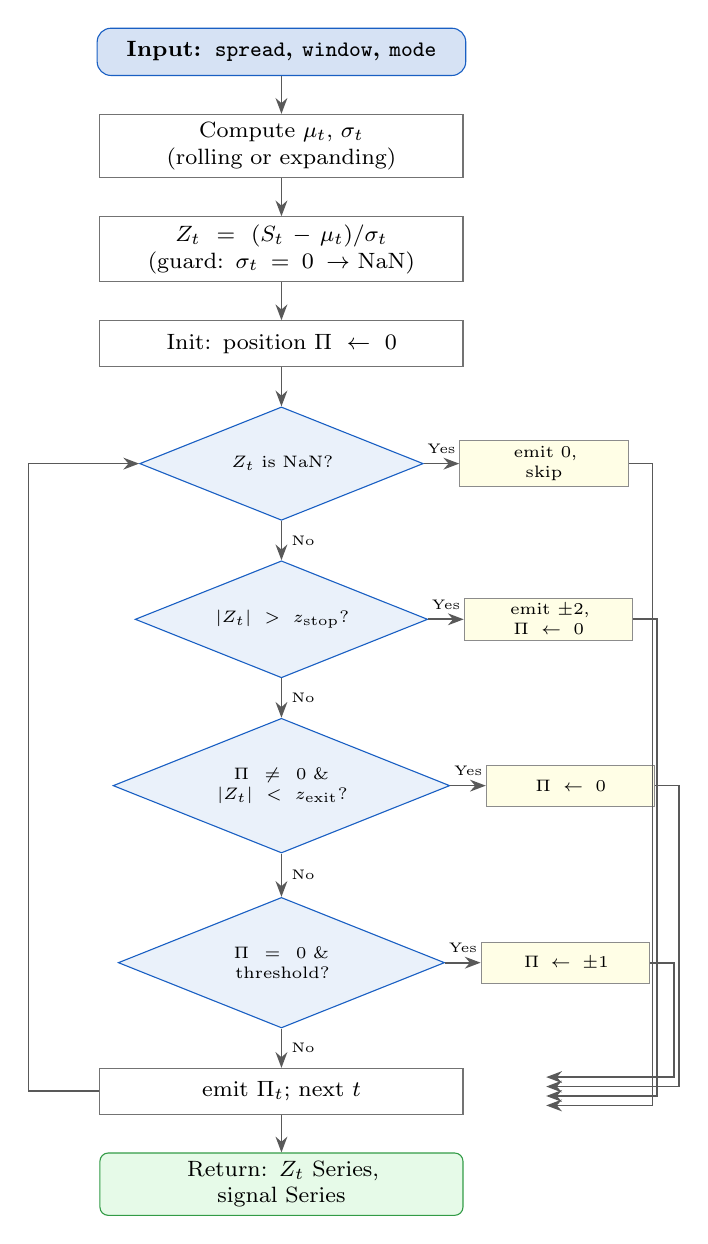
\begin{tikzpicture}[node distance=0.48cm,
                    every node/.style={font=\scriptsize}]
  % Z-score computation
  \node (in) [fc_start]
    {Input: \texttt{spread}, \texttt{window}, \texttt{mode}};
  \node (roll) [fc_proc, below=of in]
    {Compute $\mu_t$, $\sigma_t$\\ (rolling or expanding)};
  \node (z) [fc_proc, below=of roll]
    {$Z_t = (S_t - \mu_t)/\sigma_t$\\ (guard: $\sigma_t=0\to$ NaN)};
  \node (sig) [fc_proc, below=of z]
    {Init: position $\Pi\leftarrow 0$};
  % State machine loop
  \node (d_nan) [fc_dec, below=0.5cm of sig]
    {$Z_t$ is NaN?};
  \node (skip) [fc_side, right=0.45cm of d_nan]
    {emit 0,\\ skip};
  \node (d_stop) [fc_dec, below=0.5cm of d_nan]
    {$|Z_t|>z_{\text{stop}}$?};
  \node (stop_act) [fc_side, right=0.45cm of d_stop]
    {emit $\pm 2$,\\ $\Pi\leftarrow 0$};
  \node (d_exit) [fc_dec, below=0.5cm of d_stop]
    {$\Pi\neq 0$ \&\\ $|Z_t|<z_{\text{exit}}$?};
  \node (exit_act) [fc_side, right=0.45cm of d_exit]
    {$\Pi\leftarrow 0$};
  \node (d_entry) [fc_dec, below=0.55cm of d_exit]
    {$\Pi=0$ \&\\ threshold?};
  \node (entry_act) [fc_side, right=0.45cm of d_entry]
    {$\Pi\leftarrow\pm 1$};
  \node (emit) [fc_proc, below=0.5cm of d_entry]
    {emit $\Pi_t$; next $t$};
  \node (out) [fc_out, below=of emit]
    {Return: $Z_t$ Series,\\ signal Series};

  \draw[arr] (in)--(roll); \draw[arr] (roll)--(z);
  \draw[arr] (z)--(sig); \draw[arr] (sig)--(d_nan);
  \draw[arr] (d_nan)--node[above,font=\tiny]{Yes}(skip);
  \draw[arr] (d_nan)--node[right,font=\tiny]{No}(d_stop);
  \draw[arr] (d_stop)--node[above,font=\tiny]{Yes}(stop_act);
  \draw[arr] (d_stop)--node[right,font=\tiny]{No}(d_exit);
  \draw[arr] (d_exit)--node[above,font=\tiny]{Yes}(exit_act);
  \draw[arr] (d_exit)--node[right,font=\tiny]{No}(d_entry);
  \draw[arr] (d_entry)--node[above,font=\tiny]{Yes}(entry_act);
  \draw[arr] (d_entry)--node[right,font=\tiny]{No}(emit);
  \coordinate (join_entry) at ([xshift=1.05cm,yshift=0.18cm]emit.east);
  \coordinate (join_exit)  at ([xshift=1.05cm,yshift=0.06cm]emit.east);
  \coordinate (join_stop)  at ([xshift=1.05cm,yshift=-0.06cm]emit.east);
  \coordinate (join_skip)  at ([xshift=1.05cm,yshift=-0.18cm]emit.east);
  \draw[arr] (entry_act.east) -- ++(0.30,0) |- (join_entry);
  \draw[arr] (exit_act.east)  -- ++(0.30,0) |- (join_exit);
  \draw[arr] (stop_act.east)  -- ++(0.30,0) |- (join_stop);
  \draw[arr] (skip.east)      -- ++(0.30,0) |- (join_skip);
  \draw[arr] (emit)--(out);
  % Loop back arrow
  \draw[arr] (emit.west) -- ++(-0.9,0) |- (d_nan.west);
\end{tikzpicture}
}
\caption{State machine for \texttt{ZScore.generate\_signals()}.
The loop-back arrow advances $t$ at each iteration.}
\label{fig:zscore_flow}
\end{figure}

%=============================================================================
\section{Worked Example}
%=============================================================================

\begin{tcolorbox}[exbox={Setup}]
$S = [0.05, -0.10, 0.08, -0.06, 0.12, -0.03, 0.07]$\\
Mode: rolling, $W=3$, $z_e=1.0$, $z_x=0.3$, $z_s=2.0$.
\end{tcolorbox}

\begin{center}{\small
\begin{tabular}{@{}ccccc@{}}
\toprule
$t$ & $S_t$ & $\mu_t$ & $\sigma_t$ & $Z_t$\\\midrule
3 & 0.08 & 0.010 & 0.076 & 0.92\\
4 & $-$0.06 & 0.007 & 0.092 & $-$0.73\\
5 & 0.12 & 0.047 & 0.093 & 0.79\\
6 & $-$0.03 & 0.010 & 0.076 & $-$0.52\\
7 & 0.07 & 0.053 & 0.076 & 0.23\\
\bottomrule
\end{tabular}
}\end{center}

\noindent With $z_e=1.0$: no entry triggers (all $|Z_t|<1.0$).\\
With $z_e=0.7$: $Z_3=0.92>0.7$ triggers SHORT at $t=3$.

\begin{tcolorbox}[resultbox={Interpretation}]
No signal fired at $z_e=2.0$ for this 7-point sample ---
the spread is mild.  This is expected: with a half-life of $\sim$1
observation, the spread oscillates rapidly but with small amplitude,
giving $Z_t$ values below the entry threshold.
\end{tcolorbox}

%=============================================================================
\section{Python Implementation}
%=============================================================================

\begin{tcolorbox}[codebox={Z-score computation}]
\begin{lstlisting}[style=pythonplain]
def compute(self) -> pd.Series:
    s = self._spread
    if self.mode == "rolling":
        roller = s.rolling(window=self.window,
                    min_periods=self.min_periods)
        self._mu    = roller.mean()
        self._sigma = roller.std(ddof=1)
    else:  # expanding
        exp = s.expanding(min_periods=self.min_periods)
        self._mu    = exp.mean()
        self._sigma = exp.std(ddof=1)
    sigma_safe = self._sigma.replace(0.0, np.nan)
    self._zscore = ((s - self._mu) / sigma_safe
                   ).rename("zscore")
    return self._zscore
\end{lstlisting}
\end{tcolorbox}

\begin{tcolorbox}[codebox={State-machine signal (inner loop)}]
\begin{lstlisting}[style=pythonplain]
for t in range(n):
    zt = z[t]
    if np.isnan(zt): sig[t]=0; continue
    # stop loss
    if abs(zt) > self.stop_z:
        sig[t] = 2*int(np.sign(zt))
        position = 0; continue
    # exit
    if position != 0 and abs(zt) < self.exit_z:
        position = 0
    # entry
    if position == 0:
        if zt < -self.entry_z:   position = 1
        elif zt > self.entry_z:  position = -1
    sig[t] = position
\end{lstlisting}
\end{tcolorbox}

%=============================================================================
\section{Connection to Kalman Filter}
%=============================================================================

\begin{tcolorbox}[notebox={ZScore $\to$ Kalman Interface}]
The Kalman Filter in \texttt{complete\_kalman\_filter.py} uses the
\emph{raw} spread $S_t$ (not $Z_t$) as its observation.  However,
the Z-score is useful as a \emph{post-filter} normalisation:
\begin{enumerate}\setlength\itemsep{1pt}
  \item Kalman produces dynamic spread $s_t = Y_t - \hat\beta_t X_t$.
  \item \texttt{ZScore(s\_kalman, window=2*tau)} normalises it.
  \item $Z_t$ from Kalman is more stable as $\beta_t$ adapts.
\end{enumerate}
Recommended: use Kalman spread with rolling Z-score for live signals.
\end{tcolorbox}

%=============================================================================
\section{Threshold Selection Guide}
%=============================================================================

\begin{center}
{\small
\begin{tabular}{@{}p{1.4cm}p{1.4cm}p{2.6cm}@{}}
\toprule
Parameter & Default & Guideline\\
\midrule
$z_{\text{entry}}$ & 2.0 & Lower=more trades, less edge\\
$z_{\text{exit}}$ & 0.5 & Higher=exit earlier, less profit\\
$z_{\text{stop}}$ & 3.5 & Must $> z_{\text{entry}}$; 3$\sigma$ is standard\\
$W$ (window) & $2\tau$ & From \texttt{half\_life.estimate()}\\
mode & rolling & Use expanding for $\tau>120$\\
\bottomrule
\end{tabular}
}
\end{center}

\end{document}
